%\subsection{Estimating Bathymetry}

In this Section, we describe some experimental results with simulated and real data using few existing nonlinear optimization tools that we used in our preliminarily experiments (see Section \ref{inv_techniques}). Note that our forward model is nonlinear as described in Section \ref{forwardproblem} and it can not be written as a matrix equation system. Therefore, in this Bathymetry inversion, we can not use any inverting method where it needs forward operator as a explicit matrix operator (e.g., \verb|tikhonov| and  \verb|lsqnonneg|     
 Matlab\textsuperscript{\textregistered} functions need forward operator as a matrix). Moreover, the bounds of the true Bathymetry in the interested near shore region is known to be $[0m, 11m]$. Therefore, we picked the inverse solvers that enables us to incorporate that prior knowledge too. 

\subsection{Simulated Data}
In this study, Gaussian noise corrupted simulated wave numbers (see Section \ref{Gaussian_noise} for more details) are generated by 
\begin{equation}
\mathbf{k}_s = A(\mathbf{h}_t) + \mathcal{N}(0, \nu^2),
\end{equation}
where $A(\cdot)$ represents the nonlinear forward operator defined in Section \ref{forwardproblem}, $\mathbf{h}_t \in \mathbb{R}_+^n$ is the true Bathymetry vector, and $\mathcal{N}(0, \nu^2)$ is a additive Gaussian noise vector with standard deviation $\nu$, generated in the Matlab\textsuperscript{\textregistered} by $\nu \cdot $\verb| randn(n,1)|. we manufactured wave numbers $\mathbf{k}_s$ for two different grid resolutions, i.e., 10m and 25m (see Fig. \ref{Simulated10m} and \ref{Simulated25m} respectively), to test and tune our inverse methods before working with actual measurements. 



\begin{figure}[H]
\center
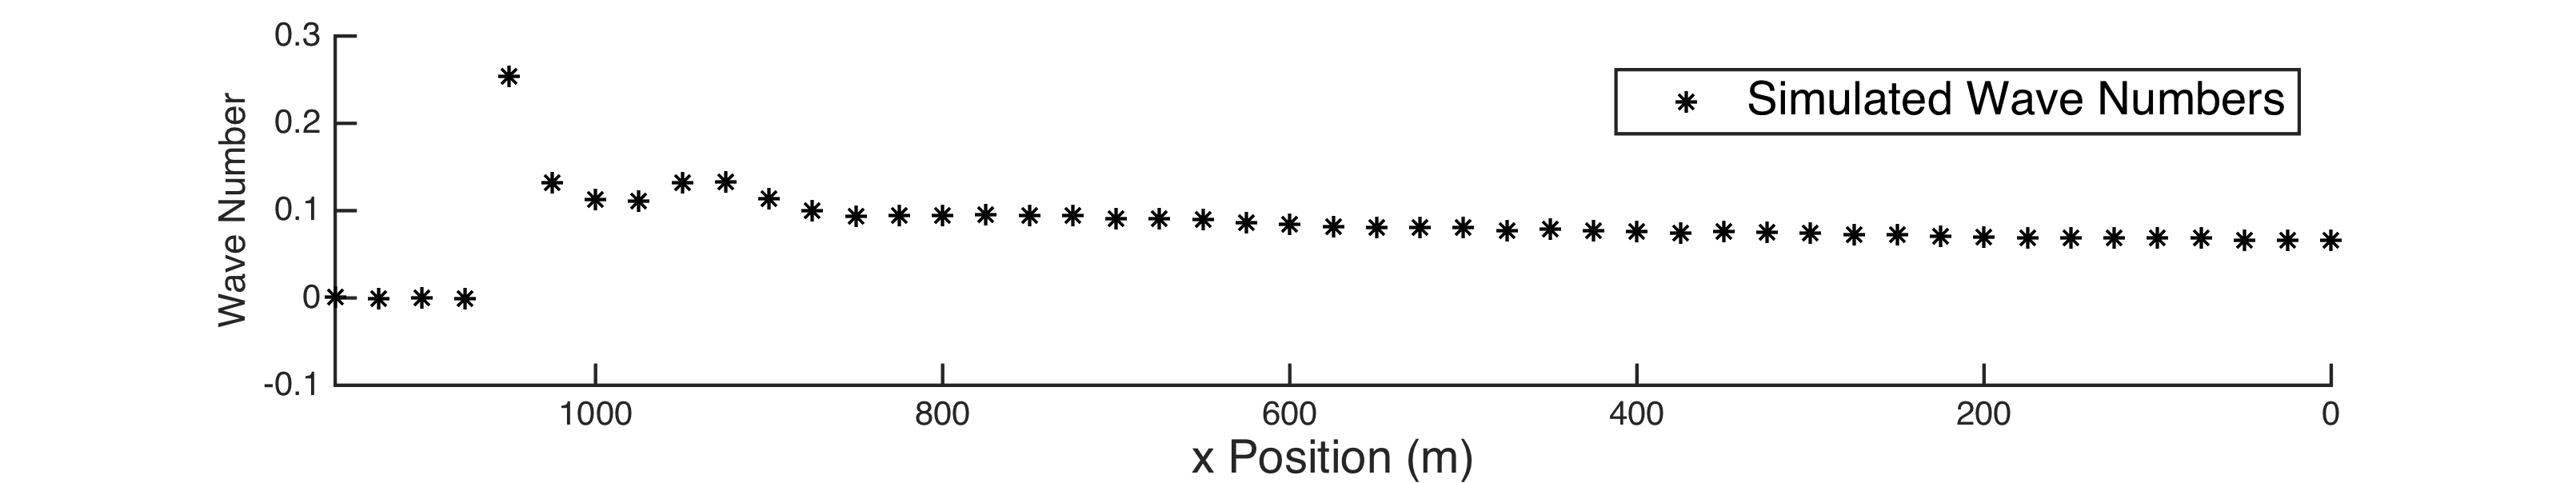
\includegraphics[scale=0.6]{img/simulated_data_k25m.png} 
\caption{1\% noisy ($\nu = 10^{-3}$) simulated wave numbers $(k)$ with 25m grid resolution. Noise (\%) = $\|A(\mathbf{h}_t) -  \mathbf{k}_s\| / \|  \mathbf{k}_s \| \cdot 100$.}
\label{Simulated25m}
\end{figure}

\begin{figure}[H]
\center
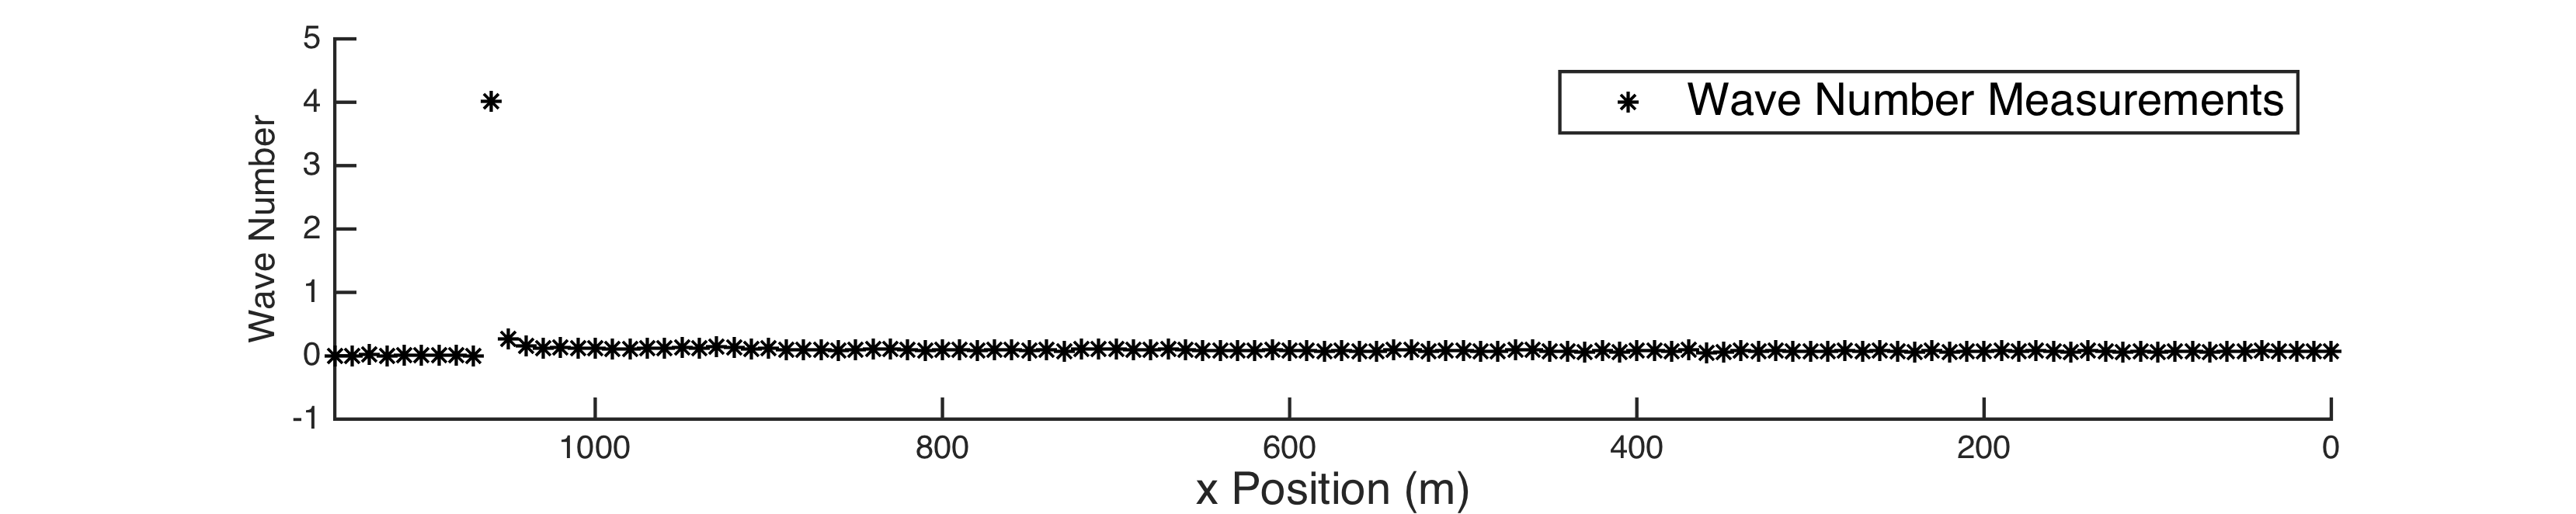
\includegraphics[scale=0.6]{img/simulated_data_k10m.png} 
\caption{2.5\% ($\nu = 10^{-2}$) noisy simulated wave numbers $(k)$ with 10m grid resolution. Noise (\%) = $\|A(\mathbf{h}_t) -  \mathbf{k}_s\| / \|  \mathbf{k}_s \| \cdot 100$. }
\label{Simulated10m}
\end{figure}


\subsection{Real Data}\label{realData}


Measured wave numbers $\mathbf{k}_m$ (see Fig. \ref{RealData_oct09}) by US Army Corps of Engineers (USACE) at the field research facilities in Duck, NC on 09th October 2015  is used to approximate the true bathymetry using different inversion schemes. Note that the measured wave numbers near the shore (x Position $>$ 1050m) and the deep end (x Position $<$ 350m) are not available for our numerical experiments. 

\begin{figure}[H]
\center
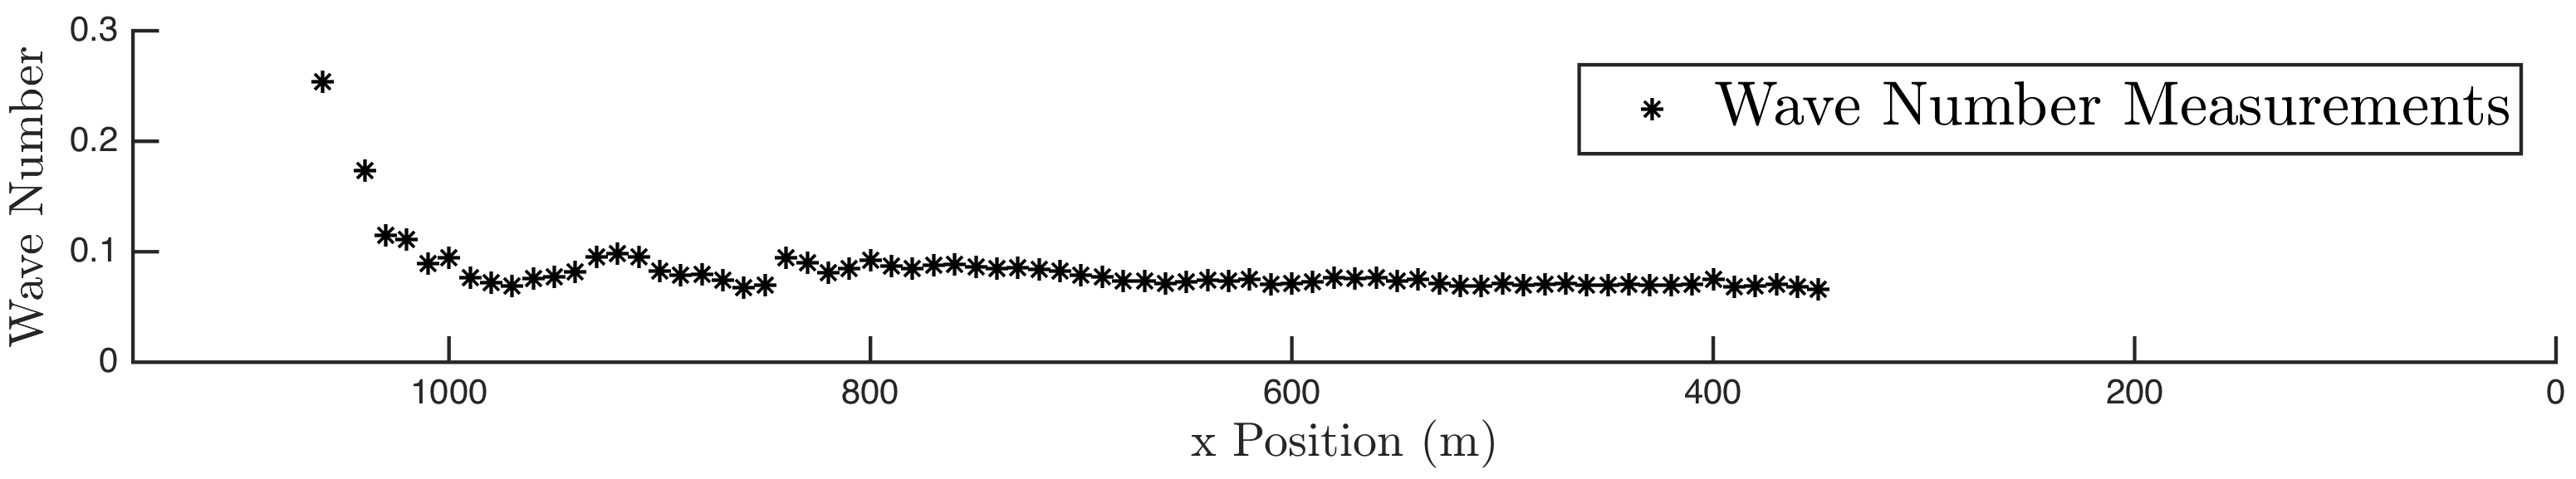
\includegraphics[scale=0.5]{img/real_data_k_Oct09.png} 
\caption{Real measurements of wave numbers $(k)$ on the 09th October 2015 at 21:59 by the US. Army Corps of Engineers (USACE) Engineer Research and Development Center (ERDC).}
\label{RealData_oct09}
\end{figure}




\subsection{Ordinary Least-Squares Fitting}
Here, we approximate the unknown bathymetry by solving the following optimization problem:
\begin{equation}\label{LS-BC}
\mathbf{\hat{h}}= \underset{\mathbf{0} \preceq \mathbf{h} \preceq \mathbf{11} }{\arg \min} \ \  \|  A(\mathbf{h}) -  \mathbf{k} \|_2^2.
\end{equation}
In particular, here we modify the ordinary least squares problem in \eqref{LS} to a bounded constrained optimization problem to incorporate the known bathymetry bounds. Based on the preliminary studies and referring the Matlab documentation, we decided to use the Matlab's \verb|lsqnonlin| function to solve this problem \eqref{LS-BC} for the simulated and real $\mathbf{k}$ measurements. According to the Matlab documentation, here we have two algorithm choices: \textit{trust-region-reflective} (default) or \textit{Levenberg-Marquardt}. However, the Levenberg-Marquardt algorithm does not handle bound constraints. Therefore, we use the trust-region-reflective algorithm (See \cite{trustregion} for more details regarding the algorithm) inside the \verb|lsqnonlin| function to recover the unknown depth parameter. Rather than input the sum of squares of the objective function in \eqref{LS-BC} to the \verb|lsqnonlin| function, it requires a user-defined vector-valued function $f(\mathbf{h}) = A(\mathbf{h}) -  \mathbf{k}$ as the function argument along on the boundary conditions. 

\begin{figure}[H]
\center
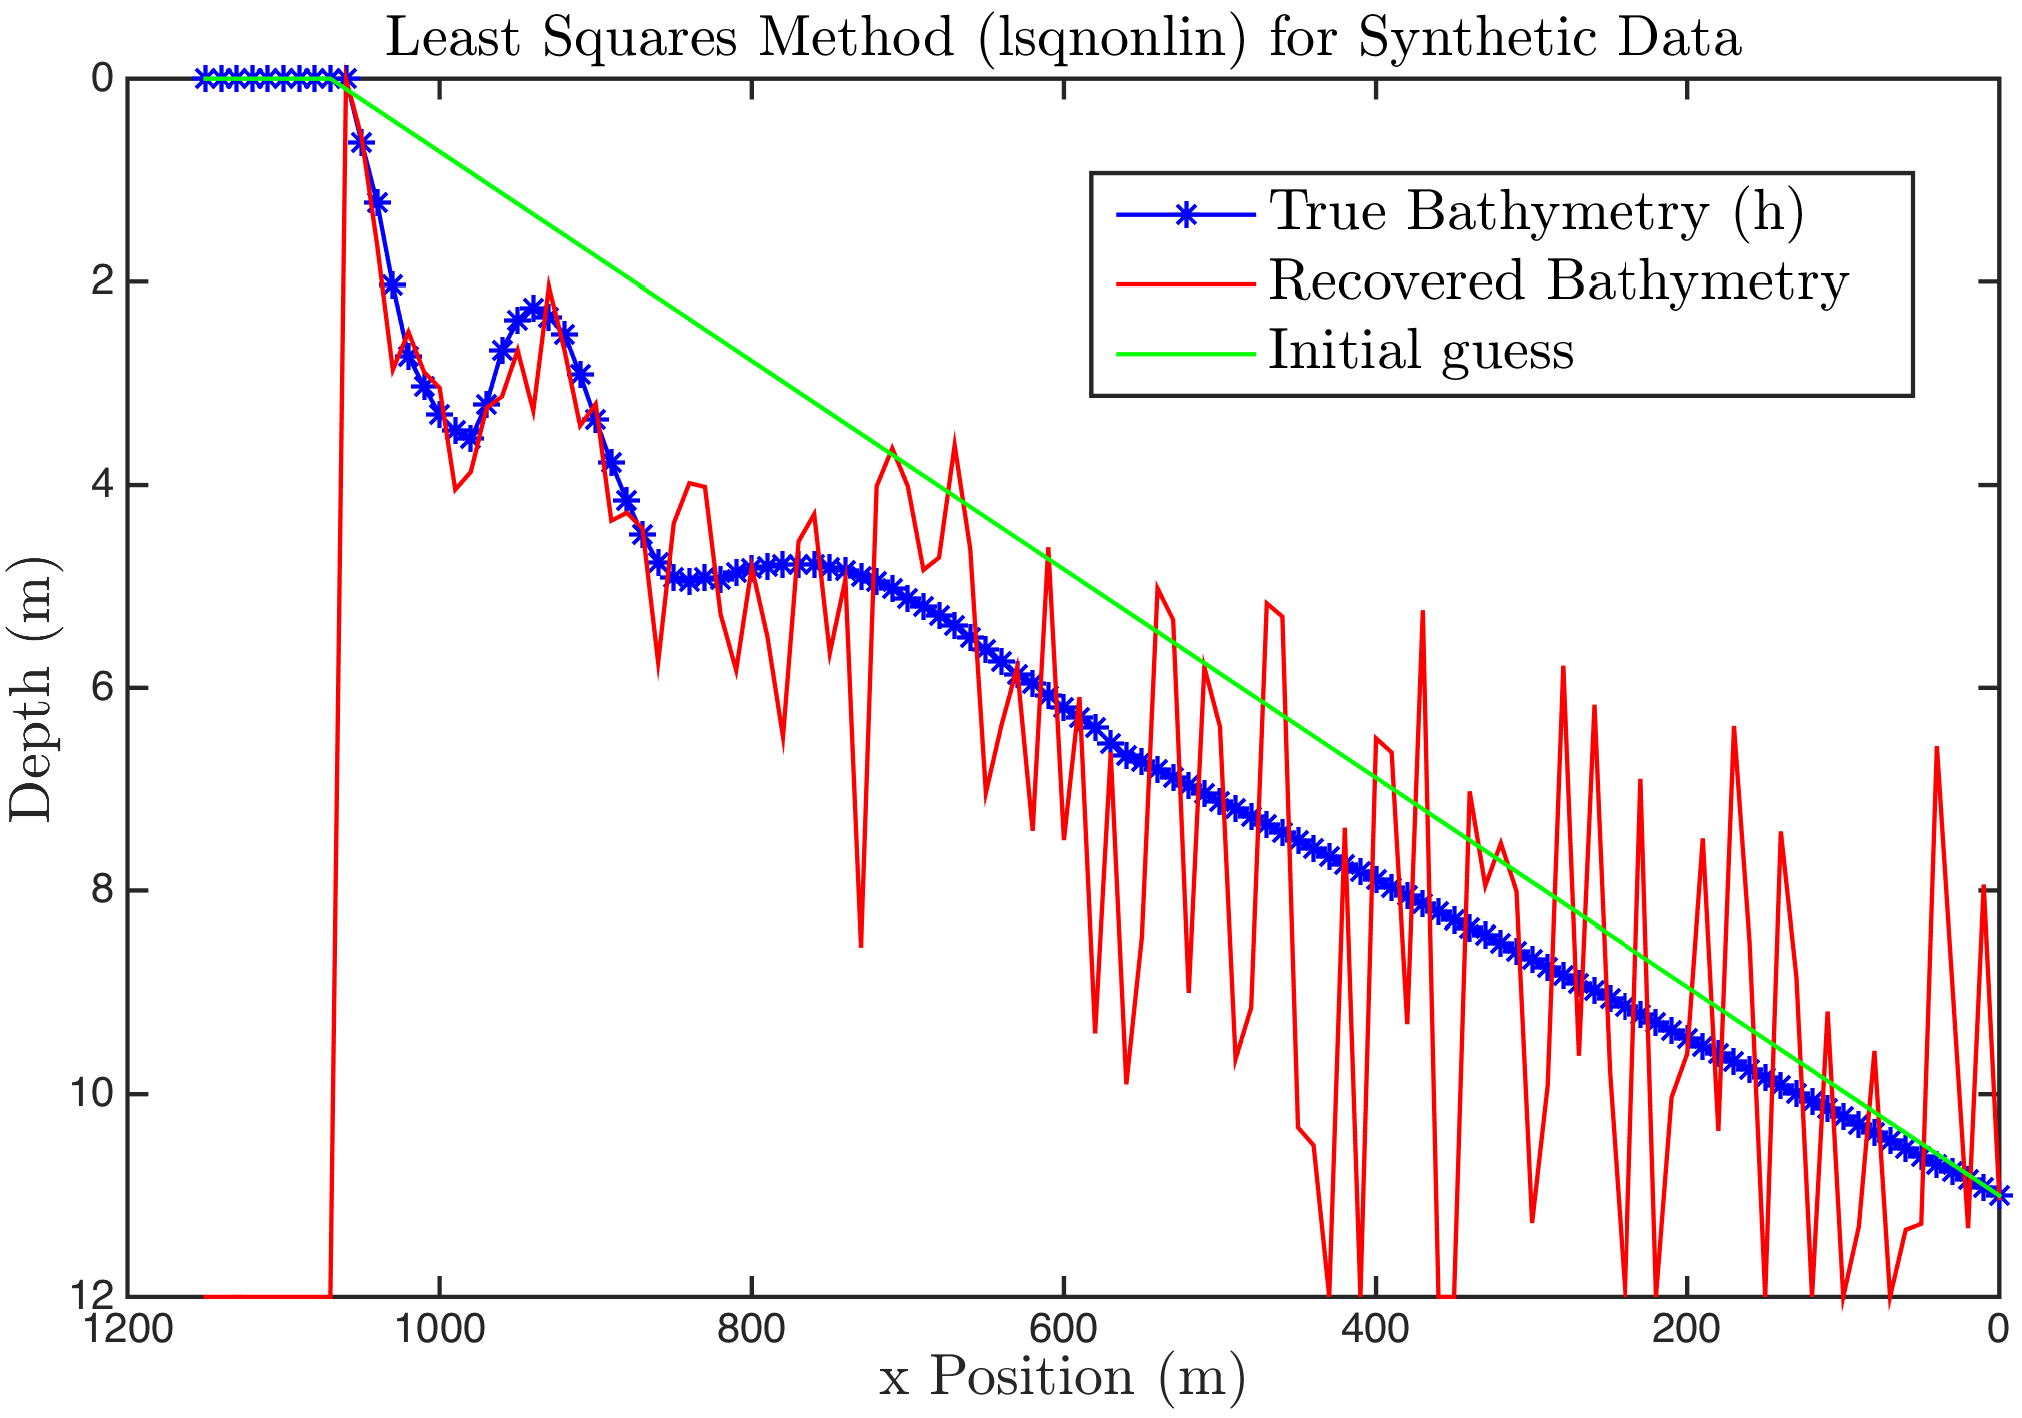
\includegraphics[scale=0.6]{img/lsqnonlin_simulated_10m.png} %plot20 
\caption{Ordinary least-squares reconstruction of depth $\mathbf{h}$ using the simulated data.}
\label{lsqnonlin_simulated}
\end{figure}
First, we run the \verb|lsqnonlin| function on the synthetic data $\mathbf{k}_s$ with 10m grid resolution. As we expected, the least-squares method captured the most interesting and important sand bar near the shoreline (see Fig. \ref{lsqnonlin_simulated} from 800m to 1000m area). However, the recovered depth is unstable from the 600m to the deep-end due to the ill-conditioned nature of the nonlinear forward operator. 

%Note that a linear function is used as the initial guess for this numerical method  and which is represented in a green color line. 
\begin{figure}[H]
\center
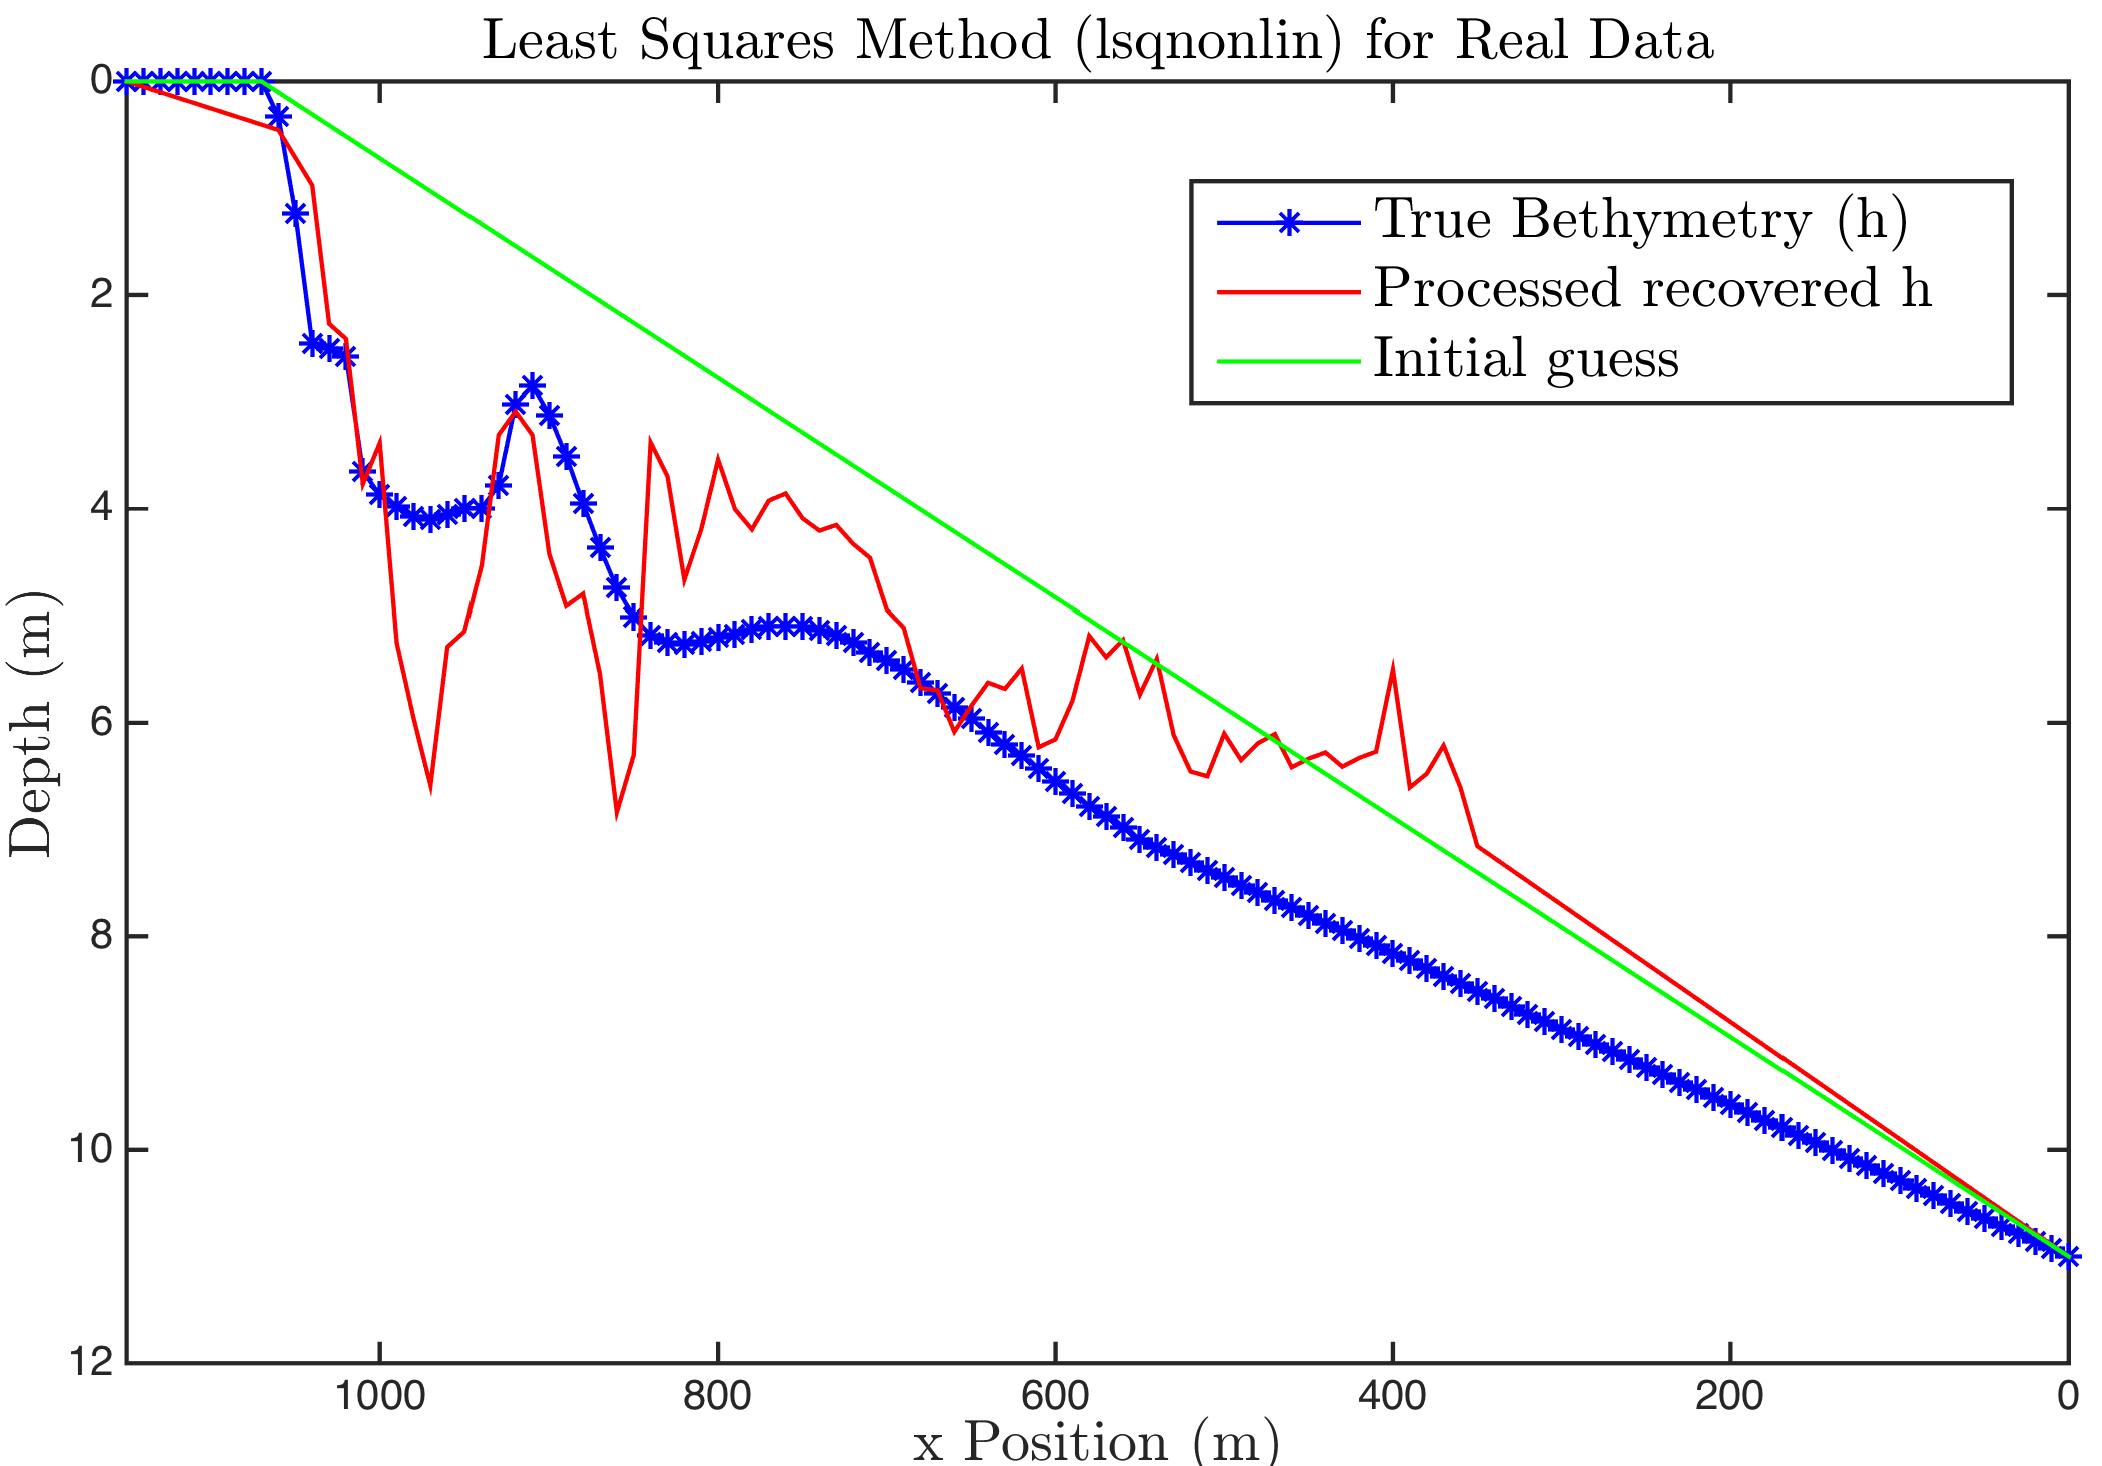
\includegraphics[scale=0.6]{img/lsqnonlin_real_data_oct09.png} %plot20 
\caption{Ordinary least-squares reconstruction of the depth $\mathbf{h}$ using the real data.}
\label{lsqnonlin_real}
\end{figure}

After comfortable with working on the synthetic data, the real wave number measurements that we discussed in Section \ref{realData} are used with the same Matlab's \verb|lsqnonlin| optimizer. In this reconstruction, we were able to capture the near-shore topography including the sand bar with $53\%$ root mean square error (see Fig. \ref{lsqnonlin_real}). Specifically, here we have interpolated and processed the depth reconstruction based on the missing measurement locations. 


\subsection{Tikhonov Regularization} \label{TickReg}

In order to get more stable solution than the ordinary least squares solution in Fig. \ref{lsqnonlin_simulated}, we solve the following Tikhonov regularization

\begin{equation}\label{LS-regBC}
\mathbf{\hat{h}} = \underset{\mathbf{0} \preceq \mathbf{h} \preceq \mathbf{11}}{\arg \min} \ \ \|  \mathbf{A}(\mathbf{h}) -  \mathbf{d} \|_2^2  +  \alpha \| \mathbf{h}\|_2^2,
\end{equation}


\begin{figure}[H]
\center
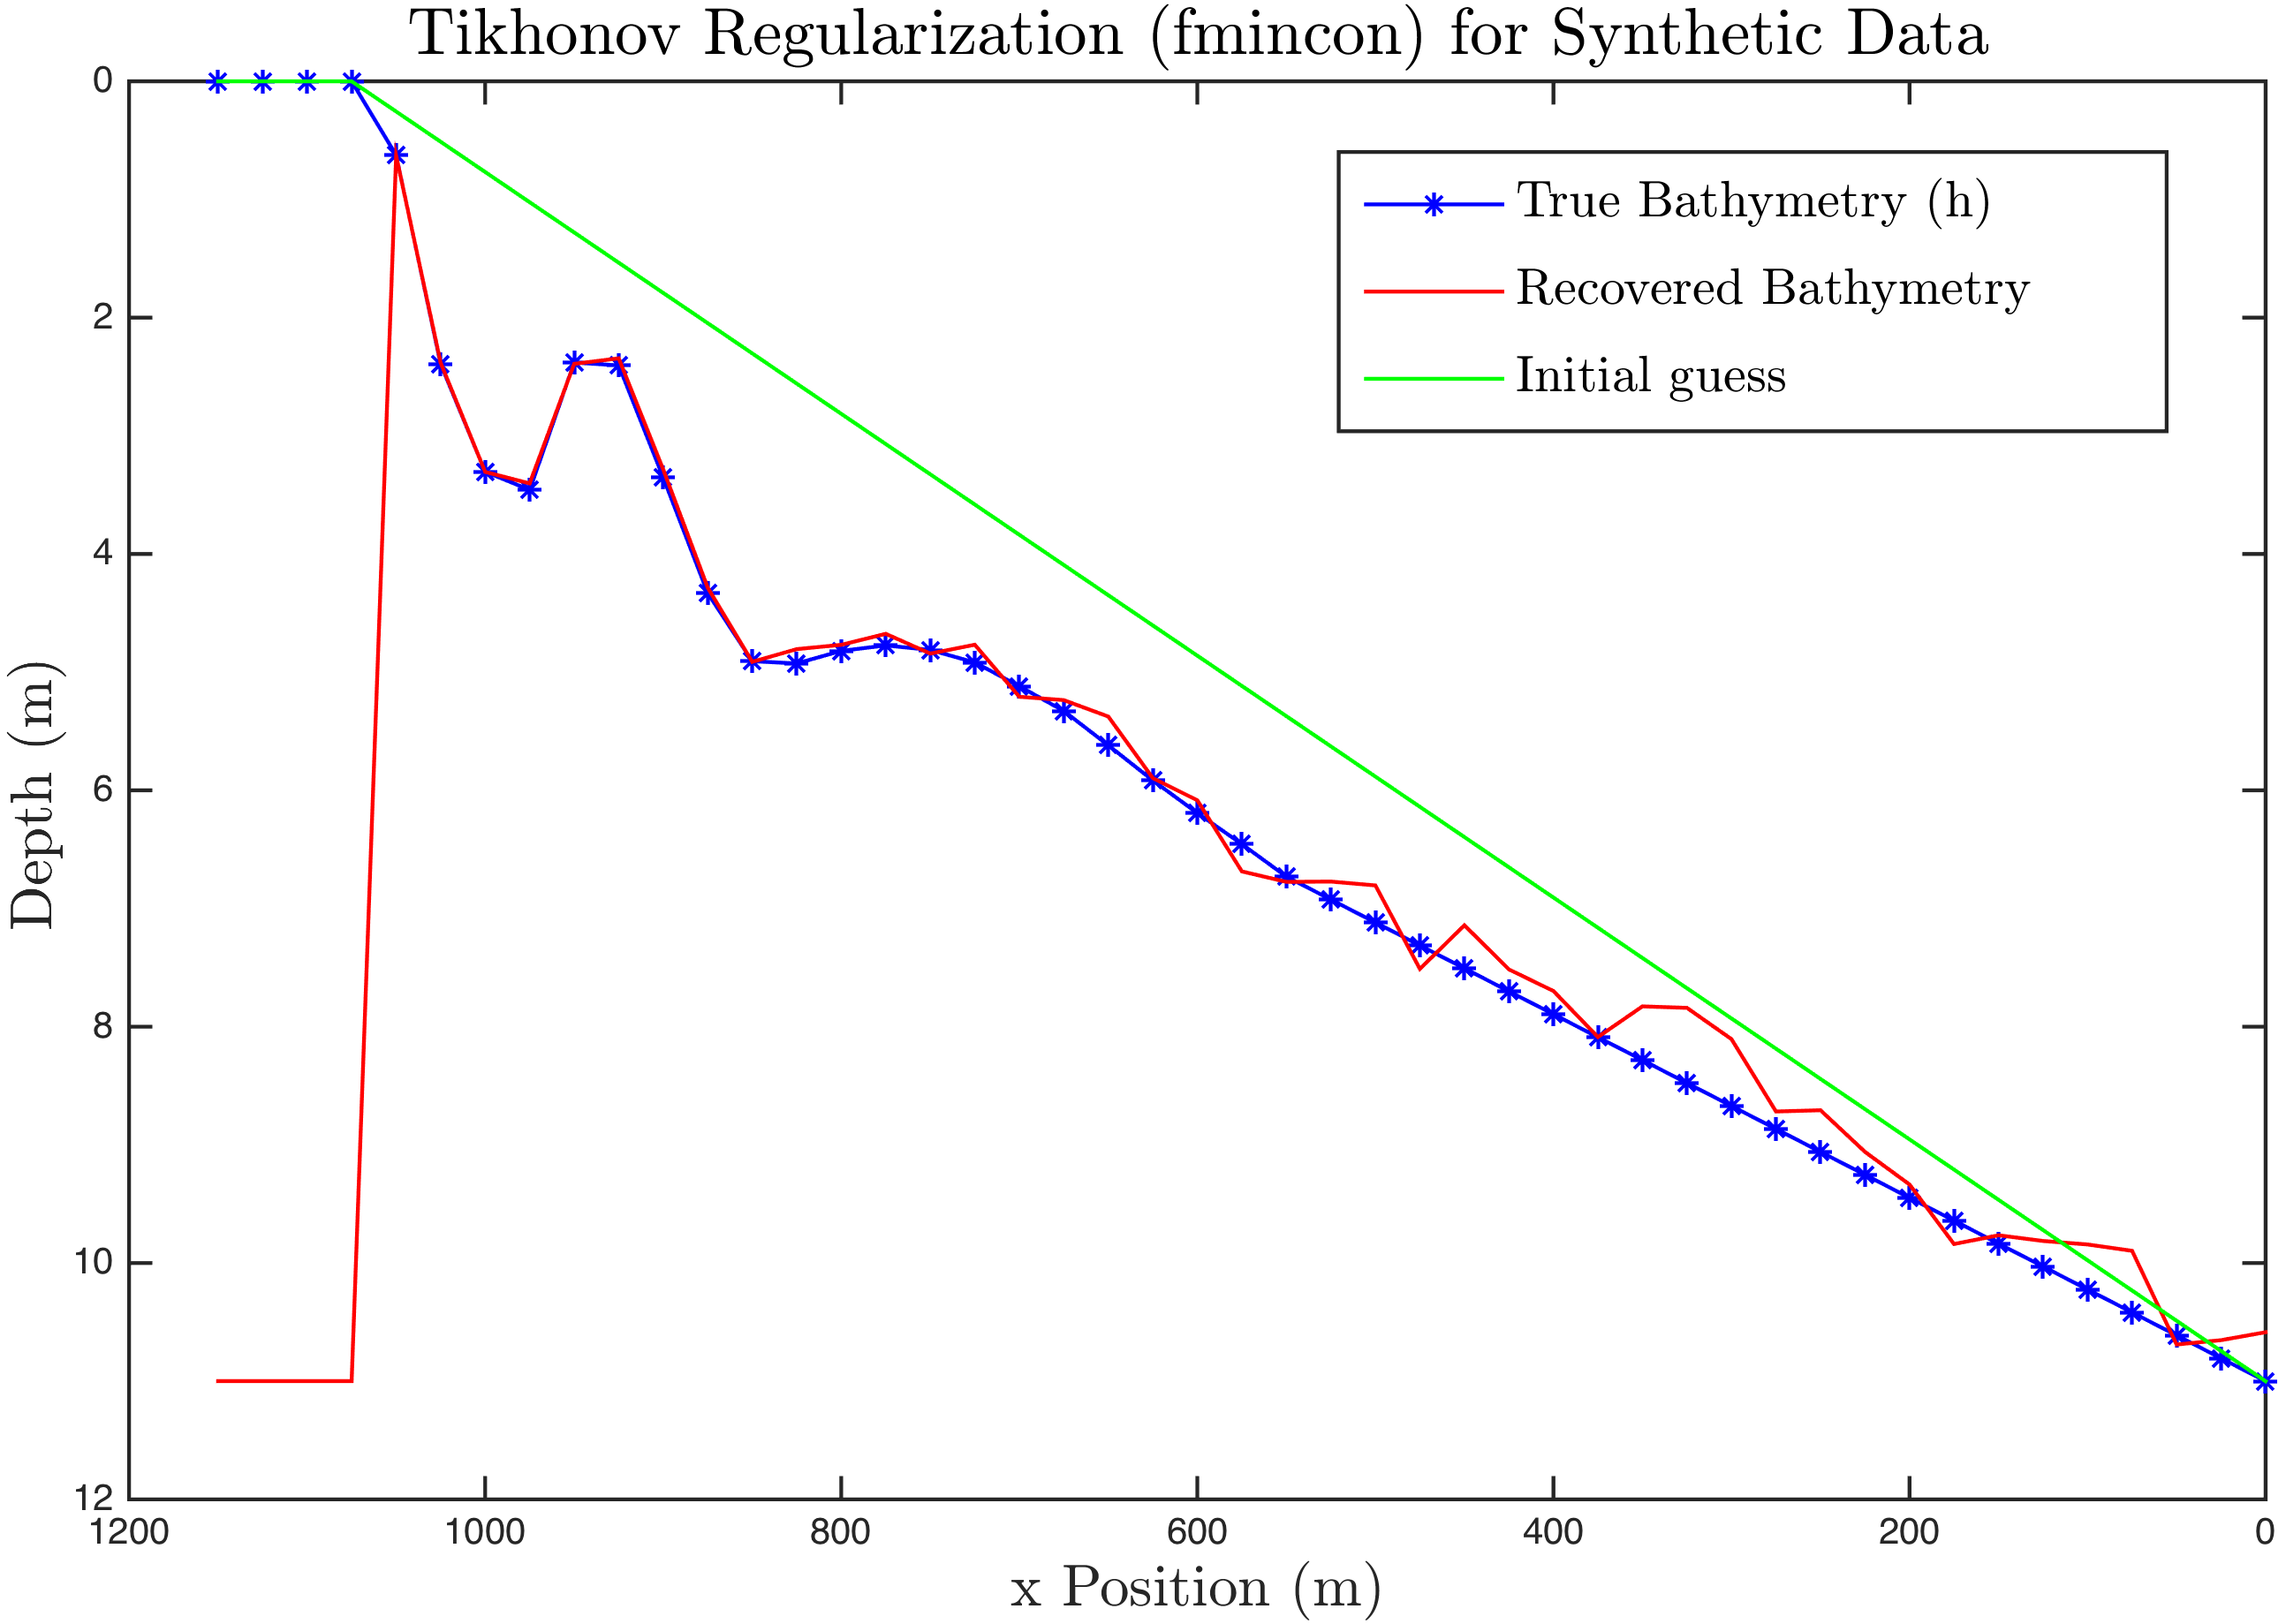
\includegraphics[scale=0.47]{img/fmincon_simulated_25_new.png} %plot20 
\caption{fmincon method reconstruction of depth $\mathbf{h}$ using the simulated data.}
\label{fmincon_simulated}
\end{figure}

\begin{figure}[H]
\center
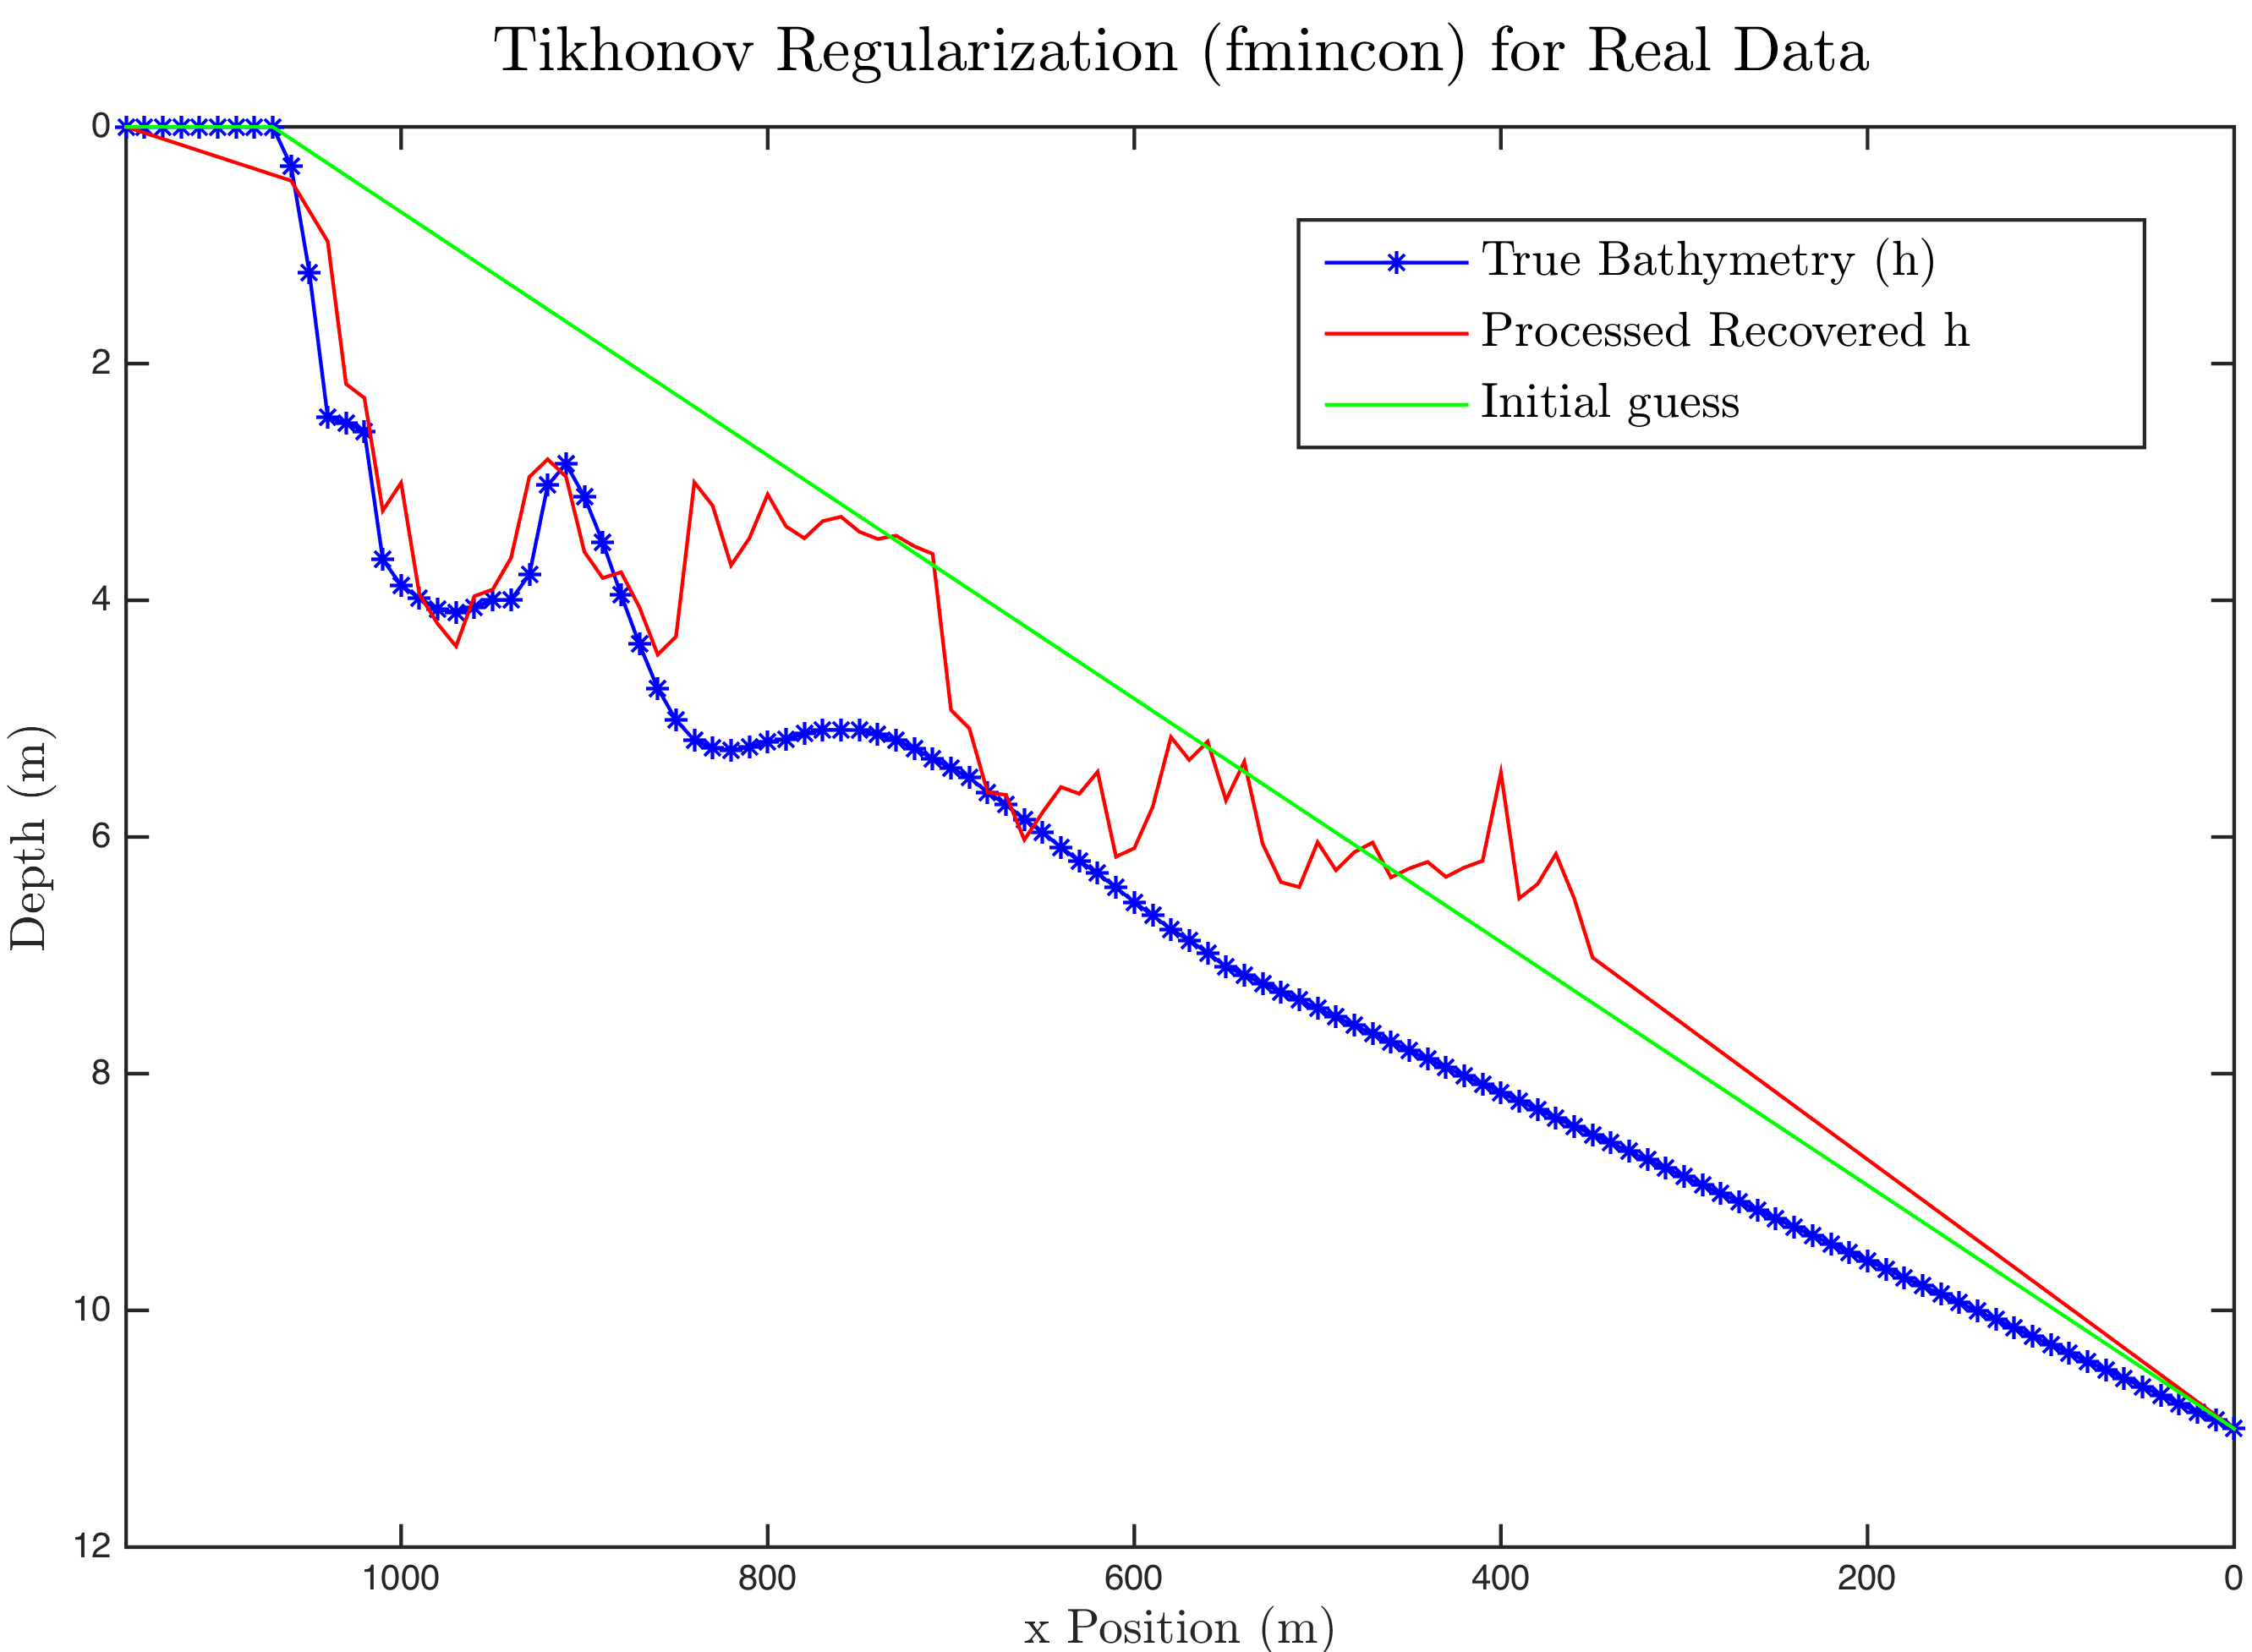
\includegraphics[scale=0.46]{img/fmincon_real_data_oct09.png} %plot20 
\caption{fmincon method reconstruction of depth $\mathbf{h}$ using the simulated data.}
\label{fmincon_simulated}
\end{figure}

